\documentclass[11pt]{article}
\usepackage{url}
\usepackage{latexsym}
\usepackage[top=1in, bottom=1.25in, left=1.25in, right=1.25in]{geometry}
\usepackage[backend=bibtex, style=alphabetic, citestyle=alphabetic]{biblatex}
\usepackage{graphicx}
\renewcommand*\rmdefault{ppl}

\usepackage{mathtools}

% Bold math
\def \aa {\mathbf{a}}
\newcommand{\bb}[0]{\mathbf{b}}
\newcommand{\ee}[0]{\mathbf{e}}
\newcommand{\ff}[0]{\mathbf{f}}

\newcommand{\scriptA}[0]{\mathcal{A}}

% argmax
\DeclareMathOperator*{\argmax}{argmax ~}

\addbibresource{references.bib}

\title{A Comparison of Phrase-Based Statistical Models for Machine Translation}

\author{Brian Cristante \\
  UNC-Chapel Hill}

\date{21 April 2015}

\begin{document}
\maketitle
\begin{abstract}
    Since their introduction in the early 1990s by the IBM Candide project, 
    statistical machine translation (SMT)
    techniques have quickly supplanted rule-based systems as the state-of-the-art
    and the focus of research in the field. But how much do statistical models benefit
    from using linguistic information? In this paper, we compare
    two popular and similar kinds of translation models: phrase-based models, 
    which operate on simple $n$-grams, and hierarchical phrase-based models, 
    which operate on both words and nodes in a parse tree.
\end{abstract}

\section{Introduction}
% Problem statement: source to target language
Statistical machine translation (SMT) attempts to develop models and systems
that can translate from one language to another based on correlations observed
in a large bilingual corpus -- a dataset of human-generated translations.
The first statistical models for translation used features
only at the word level. Since then, models have been adapted to
treat commonly occurring words as a unit
and even learn grammar rules that account for the language in the training data.

The first group of models are called ``word-based models.'' These models simply infer
correlations between the surface forms in the bilingual text. If word $e$ appears together in one language
with word $f$ in the other frequently enough throughout the text, the model will infer that
$e$ and $f$ are translations of each other. While this is effective at learning a lexicon, word-based models struggle to order words
correctly and coherently. ``Phrase-based'' or ``alignment template based'' models seek to address this
by observing not just which words co-occur across the two languages, but within the same language.
So if words $e_1$ and $e_2$ appear adjacently throughout the corpus, a phrase-based model will
infer that $e_1 e_2$ is a phrase and will account for this when looking for a corresponding translation.
Even this is not powerful enough for languages with very different word orders, like English and Chinese.
We can apply the same method recursively and form phrases of phrases -- a ``hierarchical phrase-based''
or ``parse-based'' model. These models, while complex, are especially appealing because they reflect
our own grammatical theories of language.

There is no definitive way to evaluate the quality of translations, even those generated by humans.
But there are a number of dimensions on which their output may be assessed, and these dimensions
can be chosen to reflect the application of the system.
\textit{Black-box analyses} seek to gauge the quality of a translation system by simply comparing its output
to some standard.
\textit{Glass-box analyses} evaluate systems on how well they follow good systems engineering practices 
such as how easy it is to extend to other language pairs and incorporate new technology.
In order to understand the strengths and weaknesses of the flat phrase-based and hierarchical phrase-based approaches,
we will study several state-of-the-art implementations and compare them according to several black-box and glass-box criteria.


\subsection{A Brief History of Machine Translation}

Machine translation is a problem as old as the stored-program computer. In 1949, the same
year that the EDVAC was built,
a mathematician who had served as a codebreaker in wartime
proposed that the statistical methods and noisy channel model of cryptography
be used to translate natural languages \cite{weaver_memo}.
However, this statistical approach to translation was set aside, 
lacking computational power, good statistical methods, and especially good data \cite{lopez}. 
In the time since, our processors have grown exponentially in speed thanks to integrated circuits and Moore's Law
and modern operating systems are built to schedule parallelized tasks on multicore architectures.
We have sophisticated machine learning techniques like Hidden Markov Models,
Expectation-Maximization (EM), and neural networks, 
subroutine packages for mathematical optimization, and a wealth of experience from
applying these methods to other natural language problems like automatic speech recognition \cite{brown:93, och:99}.
With the Web, we have an abundant supply of bilingual corpora on which we can train our statistical models \cite{lopez}.

In the early 1990s, the IBM Candide project applied statistical methods effectively in a French-English
system \cite{brown:93}. Their 1993 paper has become the seminal work in SMT.
Its influence is so pronounced that the standard notation for strings in the source language and target language remain $\ff$ for French
and $\ee$ for English, regardless of the actual languages in the application.
But this also reflects a key hypothesis of the statistical approach: if a model is formulated without
an explicit dependence on linguistics, do the identities of the languages really matter?

\section{The Anatomy of a Translation Model}
\subsection{Alignments}
\label{desiderata}
% Example of direct translation with a dictionary + shortcomings
Imagine we are trying to translate some written text from English to Spanish.
We could try taking an English-Spanish dictionary, looking up every English word,
and writing down the corresponding Spanish term at the same position in our output sentence.
Of course this technique would not produce good translations, but why not?

First, it assumes that there is a one-to-one correspondence of words in English and Spanish.
This is generally not the case. As a common counterexample, English uses a slew of 
helping verbs like \emph{am}, \emph{has}, and \emph{will} to construe tense
while Spanish would simply change the suffix of a verb.
Idioms fall in the same category as whole phrases that ought to be treated as a single semantic unit.
Also, the model treats every uniquely spelled string as a distinct word in both the source and target languages.
This totally ignores \textit{morphology}, a language's rules for altering words to convey grammatical
and semantic information. For example, the model would see no relation between \textit{dog} and \textit{dogs}
or \textit{jump} and \textit{jumped}. Besides matters of efficient storage, this is a problem because,
in translation, the system will be able to generate only those word forms that appeared in its training data.
For a highly inflected language like Spanish, which has rich verb conjugations, it is unlikely that
all of these forms will be attested in the corpus \cite{brown:93}.

Lastly, we have assumed that the word orders of both the source and target languages are the same.
English and Spanish are both languages with Subject-Verb-Object word orders,
so this may seem like a reasonable simplification. But consider the following examples:

\bigskip

\indent\textbf{E:} ``central processing unit'' \\
\indent\textbf{S:} ``unidad central de procesamiento'' \\

\medskip

\indent\textbf{E:} ``I like John.'' \\
\indent\textbf{S:} ``Juan me gusta.''

\bigskip

The latter is an instance of \textit{thematic divergence}: when a word that is a subject in the source
language becomes the object in the target language, and vice versa, because of a difference
in the semantics of the verb used in each language. This is one of the many nuances
that undermined the original rule-based approaches to translation \cite{dorr_survey}.

% How we seek to address some of those shortcomings
The IBM Candide group discovered how to infer \textit{alignments} between
words in parallel sentences using a model informed with a large, bilingual text corpus. 
The alignments for the above examples are shown in Figure \ref{alignments}.
This method has the added advantage of not even needing a lexicon: the translations are inferred directly
from the co-occurrence of words in the text. 

The mathematics of such a method are an appropriate introduction
to the more advanced SMT models that follow.
Aside from introducing useful concepts, terminology, and notation, almost every SMT model
is formulated according to steps like those used here \cite{lopez}.

\begin{figure}
\centering
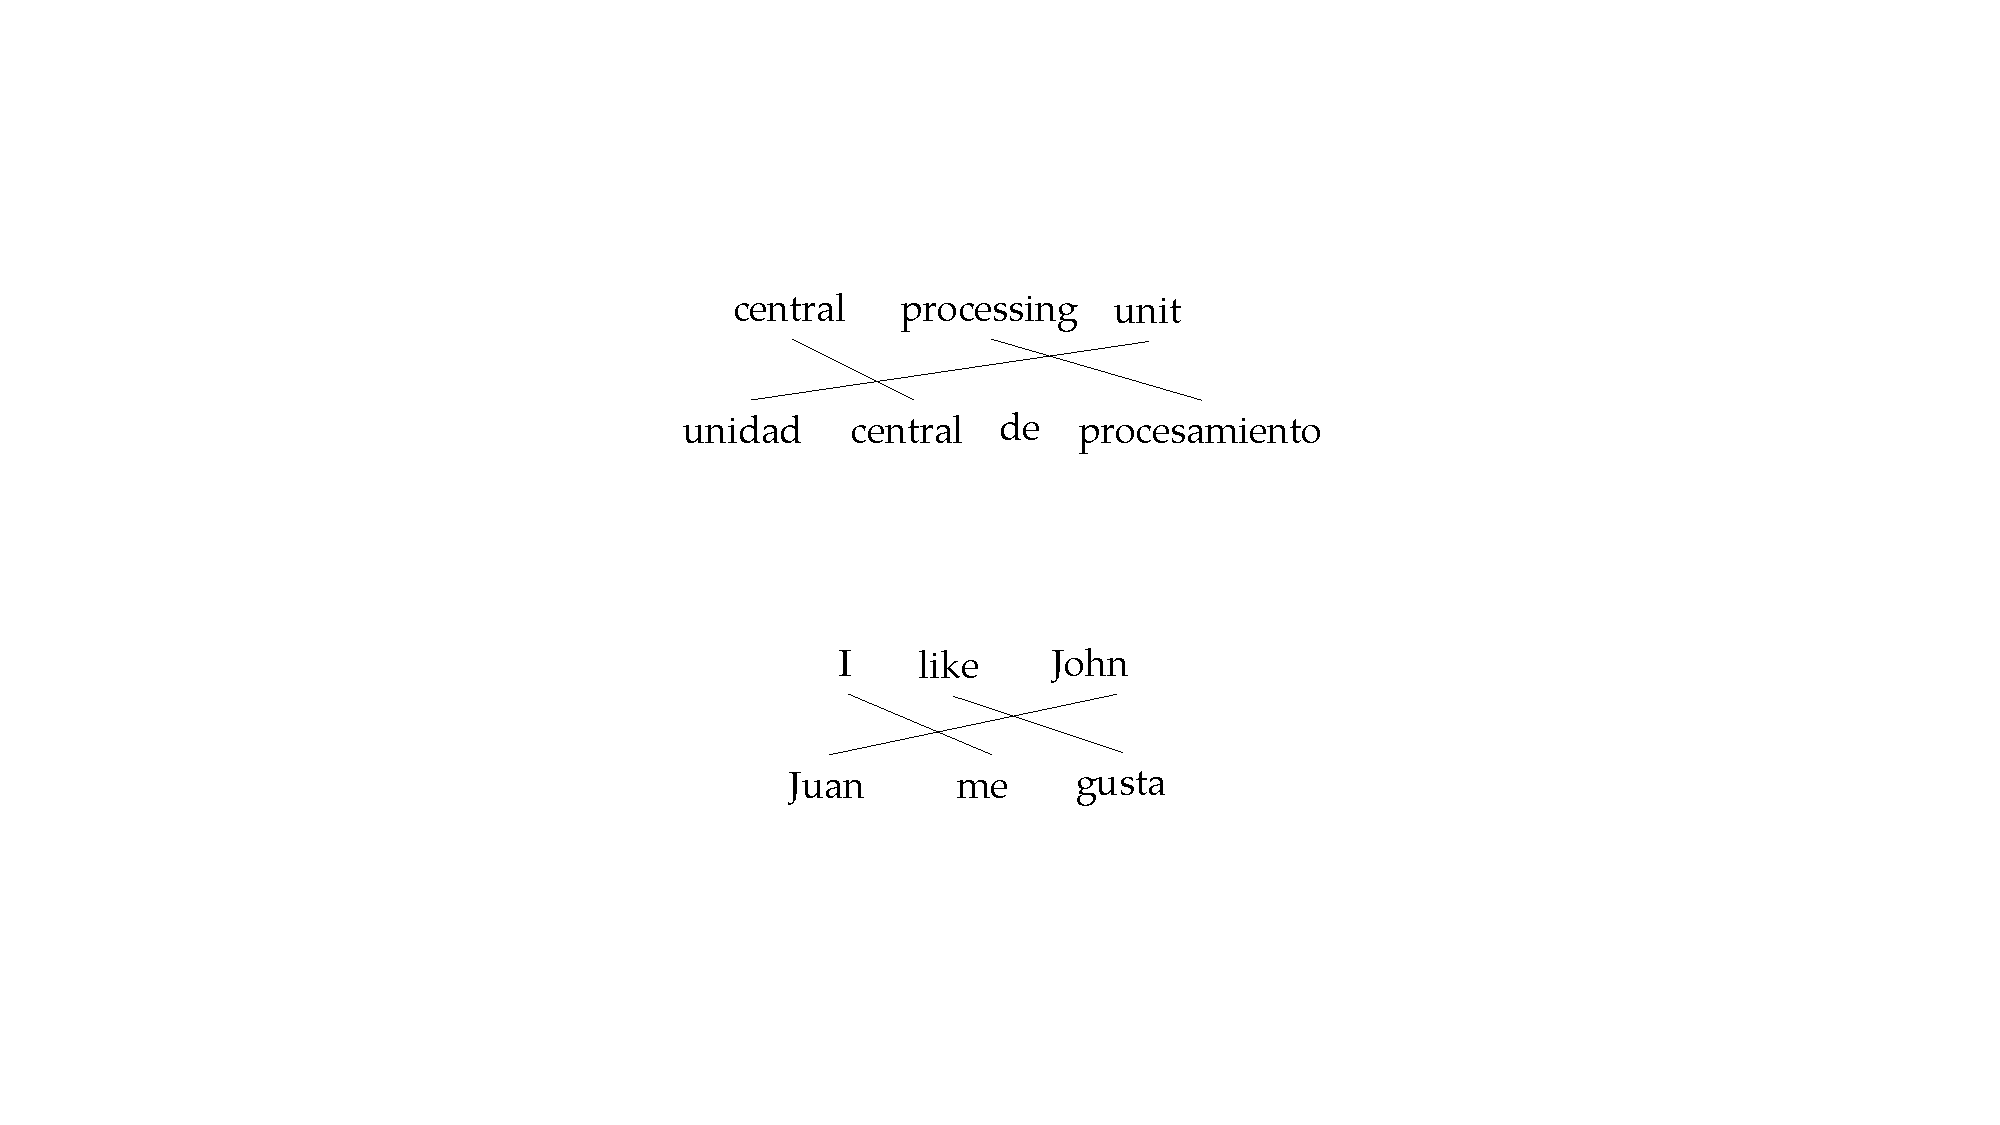
\includegraphics[trim = 300px 125px 300px 125px, scale = 0.7]{align.pdf}
\caption{In the first example, \textit{de} is not aligned to any English word. In the second example, the alignment from \textit{I} to \textit{me} maps pronouns of different case, an example of
thematic divergence \cite{dorr_survey}.}
\label{alignments}
\end{figure}

\subsection{The Fundamental Equation of Machine Translation}
This and the following sections (\ref{notation} - \ref{training}) walk through some of the content from the IBM Candide group \cite{brown:93} on formulating a basic SMT model.
The Candide system translates from French to English, trained on a corpus obtained from
the proceedings of Canadian Parliament.

% Math
Given the input, a French string $\ff$, we seek an English string $\ee$ that optimizes

\begin{equation}
    \argmax_{\ee} \Pr(\ee | \ff)
\end{equation}

Using Bayes' Rule, we can expand this to

\begin{equation} \label{fundamental}
    \argmax_{\ee} \Pr(\ee) \Pr(\ff | \ee)
\end{equation}

dropping the denominator because it does not depend on $\ee$.
Brown et al.\ \cite{brown:93} call this the ``Fundamental Equation of Machine Translation.''

Decomposing $\Pr(\ee | \ff)$ into $\Pr(\ff | \ee)$ and $\Pr(\ee)$ may seem redundant, 
but this formulation of the problem provides the robustness requisite for the translation task. 
We call $\Pr(\ff | \ee)$ the \textit{translation model} and $\Pr(\ee)$ the \textit{language model} \cite{brown:93}.
A model trained on $\Pr(\ee | \ff)$ alone
would have to correctly predict not only the correct English words in $\ee$ based on $\ff$, but
their correct order as well. 
By including $\Pr(\ee)$, it is now permissible for
the model to assign higher probabilities to sentences of correct words in the wrong order, which will
be balanced out with a low $\Pr(\ee)$. Likewise, the language model will reinforce
grammatically correct translations. Furthermore, language models are
already well-studied from other NLP tasks like automatic speech recognition and
may simply be reused here \cite{brown:93, lopez}.

This also means that, when describing translation models in the literature,
authors often speak of generating a source-language string from a target-language string,
even though the system is meant to do the opposite.
This is simply a metaphor for describing the mathematics -- in parameterizing $\Pr(\ff | \ee)$, 
the English string $\ee$ is our given. When the system is given a French string
during the translation phase, it will need to search for the English string that scores highest on this probability
(called \textit{decoding}).
This is certainly a non-trivial problem (in fact, it is NP-Hard: see \cite{knight:99}) 
but the development of better heuristics for search is orthogonal to the models discussed in this paper.


\subsection{Notation} \label{notation}
We have not been entirely clear about which linguistic constructs are represented by $\ff$ and $\ee$.
We can generally interpret them as sentences, although for some applications we may wish
to have them represent any chunk of punctuation-delimited language \cite{och:99}.
So if $f$ and $e$ are individual words in French and English respectively, let $\ff$ and $\ee$
simply be sequences of words:

\begin{align*}
    \ff &\equiv (f_1, f_2, \dotsc, f_m) \\
    \ee &\equiv (e_1, e_2, \dotsc, e_n) \\
\end{align*}

This notation proves to be powerful later on. Instead of words, each $e_i$ and $f_j$ could just as well be
phrases \cite{och:99, koehn:03}, so the same mathematical foundation for word-based models
can easily be recycled for phrase-based models.

Conceptually, alignments are many-to-many relations between source and target words (a bipartite graph) and
could be represented by a matrix of binary values. 
This model being a simple one, we shall assume that each French word aligns to exactly one English word (that may also have other French
words aligned to it) so each alignment $\aa \in \scriptA(\ee, \ff)$ is a sequence of indices:

\[
    \aa \equiv (a_1, a_2, \dotsc, a_m)
\]

where $a_j = i$ means that the French word $f_j$ is aligned to English word $e_i$ and $a_j = 0$ means that it is aligned
to no word.

Also, we need a convenient notation for subsequences.
Let $\ff_{i:j}$ represent the ``slice'' from positions $i$ to $j$ in $\ff$, and likewise for $\ee$ and $\aa$:

\begin{align*}
    \ff_{i:j} &\equiv (f_i, f_{i+1}, \dotsc, f_j) \\
    \ff_{1:m} &\equiv \ff
\end{align*}


\subsection{Parameterization}
Now we are equipped to decompose the translation model $\Pr(\ff | \ee)$ into probabilities involving
individual words and the alignments between them. 
Let $\scriptA(\ee, \ff)$ be the set of all alignments that can be drawn between the two strings.
Since only one alignment can be drawn at a time,

\begin{equation}
    \Pr(\ff | \ee) = \sum_{\aa \in \scriptA} \Pr(\ff, \aa | \ee)
\end{equation}

Recall $\ff \equiv (f_1, f_2, \dotsc, f_m)$, so $m$ is the length of the French sentence.
This length is not known beforehand, so introduce it with the product rule:

\begin{equation}
    \Pr(\ff, \aa | \ee) = \Pr(m | \ee) \Pr(\ff_{1:m}, \aa | \ee, m)
\end{equation}

Given the length, apply the chain rule to step through the source string word-by-word:

\begin{equation}
    \Pr(\ff, \aa | \ee)  = \Pr(m | \ee) \prod_{j=1}^m \Pr(f_j, a_j | f_{1:j-1}, a_{1:j-1}, m, \ee)
\end{equation}

No independence assumptions have been made yet -- this is an
exact expression obtained from the properties of probabilities.
Apply the product rule one more time to separate the joint probability on $f_j$ and $a_j$:

\begin{align}
    \Pr(f_j, a_j | \ff_{1:j-1}, \aa_{1:j-1}, m, \ee) &= \Pr(f_j | a_j, \ff_{1:j-1}, \aa_{1:j-1}, m, \ee) \Pr(\aa_j | \ff_{1:j-1}, \aa_{1:j-1}, m, \ee) \\
        &\equiv\Pr(f_j | \ff_{1:j-1}, \aa_{1:j}, m, \ee) \Pr(a_j | \ff_{1:j-1}, \aa_{1:j-1}, m, \ee)
\end{align}

This approach of decomposing probabilities using the rules of conditional probability 
is characteristic of generative models like this one \cite{lopez}.
This decomposition is motivated by the use of alignments in our model and is a good example of how to obtain a parameterized
model from the Fundamental Equation of Machine Translation (Eq. \ref{fundamental}), but different models will use different decompositions.
For example, the IBM Models 3, 4, and 5 introduce additional concepts to allow one-to-many alignments and need to rework the equations
to include these terms \cite{brown:93}.

\subsection{Independence Assumptions}

The purpose of decomposing the translation model $\Pr(\ff | \ee)$ was to obtain a set of probabilities that could be estimated
accurately from the corpus. Mathematically, there is no difference between $\Pr(\ff | \ee)$ and the expressions we have obtained,
but it is infeasible to learn a special probability for every possible French-English pair of sentences in our domain.

In fact, we have not yet done anything to change that.
Each French word's alignment ($a_j$) depends on all of the alignments that came before it ($\aa_{1:j-1}$), 
all of the French words that came before it ($\ff_{1:j-1}$),
the ultimate length of the French sentence ($m$), and the length and identity of the English sentence ($\ee$).
Each French word ($f_j$) depends on all of these things as well as the English word to which it is aligned ($a_j$).
This is too complex: there is not enough training data to accommodate every possible dependency, and the 
search space for decoding would be far too large.
The last step in setting up the model for training is to make
\textit{independence assumptions} to obtain parameters that apply more generally \cite{lopez}.

For example, we could assume that the length of the French sentence depends only on the length of the English sentence
and not on the identities of its words. Then, $\Pr(m | \ee) = \Pr(m | n)$. We could also assume that the alignments
and translations depend only on the last $k$ French words and the aligned English word and are independent of the length of the sentence, so

\begin{align*}
    \Pr(f_j |\ff_{1:j-1}, \aa_{1:j}, m, \ee) = \Pr(f_j | \ff_{j-k:j-1}, a_j, e_{a_j})
\end{align*}

This would be an example of a $k$-gram model.

\subsection{Training} \label{training}
The ultimate goal in training is to compute the maximum likelihood estimation:

\[
\argmax_{\ee} \Pr(\ee) \Pr(\ff | \ee)
\]

One problem remains: these probabilities have been expressed in terms of alignments, but the alignments between words 
cannot be observed directly in our dataset -- they are hidden variables.
This is a ``chicken-and-egg'' problem, since the translation probabilities cannot be guessed without knowing
the alignments, and the alignments cannot be inferred without knowing which words are most likely to be
translations of one another.
The solution is an iterative method known as Expectation-Maximization (EM) \cite{brown:93}.

EM requires that we have a distribution for the hidden variables, which inevitably depends on the parameters  \cite{flach_ml, murphy_ml}.
Starting from some initial guess for the parameters, compute expected values for the hidden variables 
(the E-step). This gives a set of ``complete data'' consisting of all of the observed and hidden data items.
Then, maximize the likelihood of this particular set of complete data, thereby obtaining new
values for the model's parameters (the M-step). The IBM Model 1 is a mathematically 
simple model where this maximization can be computed quickly in closed form using Lagrange multipliers,
but in general numerical methods must be used to compute the optimizing values for the parameters \cite{brown:93}.
The new parameter values are fed back in to the distributions
for the hidden variables, thus proceeding iteratively until the maximum likelihood estimation converges. 
For a non-convex likelihood function, this is a local optimum that depends on the initial guesses for the parameters \cite{flach_ml}.

Training a more complicated model with EM can be unwieldy. For this, it is helpful to have simpler versions of the model
with stronger independence assumptions. The optimal parameters for these can then be fed back as initial guesses
for EM on progressively more complicated models \cite{brown:93}. This is called \textit{bootstrapping} the model \cite{lopez, yamada_knight}.

% \subsection{A Benchmark}
% % GIZA++

\subsection{Next Steps}
% What shortcomings remain
Section \ref{desiderata} listed a number of challenges for translation that a good model needs to address.
The first was being able to express the same idea in the target language with a different number of words than in the source language.
In the first parameterization, we assumed that our alignments could be expressed by a simple sequence:

\[
    \aa \equiv (a_1, a_2, \dotsc, a_m)
\]

where each $a_j$ takes a scalar value and so each foreign word was aligned to exactly one English word. 
This can handle both one-to-one and many-to-one alignments, where multiple foreign words map to one English word. 
However, it cannot do the opposite one-to-many mapping. 

The second desideratum was that the model be sensitive to morphology. 
Even though we did not provide for this explicitly, the model is able to pick up some morphology
from the dataset. As Brown et al.\ explain, the model knows of no relationship
between \textit{eat} and \textit{ate} in English or of \textit{mange} and \textit{j'ai mang\'{e}} in French, 
but the model would still notice that \textit{eat} is correlated with \textit{mange} and
\textit{ate} with \textit{mang\'{e}}.
The cost is an increase in the size of the vocabulary
and an inability to recognize inflected forms that do not appear in the dataset.
Furthermore, without many-to-many alignments, the model would not be sensitive to the correlation
between \textit{I ate} and \textit{j'ai mang\'{e}} (= \textit{je ai mang\'{e}}), where the French auxiliary verb
\textit{ai} depends on both English words.

Another problem not considered by Brown et al.\ regarding morphology arises not in learning the alignment,
but in decoding, when we are searching for an optimal translation $\ee$ of $\ff$.
This problem appears only for certain languages and translation directions between them.
So for the sake of argument, say we are translating in the reverse direction now, from an English input to a French output.
Given the English word \textit{eat}, we have probabilities $\Pr(f | \text{``eat''})$ for each French word $f$ in our lexicon.
Depending on the context, the correct translation may be \textit{manger}, \textit{mange}, \textit{manges}, or many others, since
\textit{eat} is the verb form for many persons and tenses, both singular and plural, active, passive, and infinitive. 
But our model will be biased to the most commonly appearing French conjugation in our dataset since this will
have the highest $\Pr(f | \text{``eat''})$. The problem is asymmetric: going back to translating
from French to English, all of the aforementioned French forms will map to \textit{eat} with high probability.
Koehn supports this argument with an experiment in \cite{europarl}.

% Word salad
A particular consequence of our simplified alignment model is
``word salad'' translation, where related words fail to move around together \cite{lopez}.
This fails to meet our third criterion, that grammatical parts of a sentence can move
as units in translation.

% Phrase-based alignments will cure all ills
These remaining problems motivate the development of phrase-based models and
are the standards by which they will be judged.
The primary goal is to expand the translation model to handle many-to-many alignments.
By incorporating the context of surrounding words, we hope to more accurately predict the 
correct morphological forms of words. 
We hope that $n$-grams will give us help and a parse will give us certainty.
And, finally, we seek a way to move groups of related words cohesively in translation
to handle languages with naturally different word orderings.

\section{Phrase-Based Models}
\subsection{Aligning Phrases}
Earlier we noted that in our sentences

\begin{align*}
    \ff &\equiv (f_1, f_2, \dotsc, f_m) \\
    \ee &\equiv (e_1, e_2, \dotsc, e_n) \\
\end{align*}

the individual $e_i$ and $f_j$ could be whole phrases instead of just words. 
Words are convenient because, at least for languages written in the Latin alphabet,
each sentence has a unique segmentation into words. 
But na\"{i}vely considering all possible segmentations of a sentence into phrases is obviously infeasible
because of the huge number of possibilities.

% Och: templates (1999)
Och and Ney, in their ``template alignment models,'' propose a common-sense way to extend the IBM models to many-to-many alignments
without a combinatorial explosion or substantially changing the mathematics  \cite{och:99}. 
We can simply train our alignment model in the opposite direction 
on our bilingual corpus. When we have a many-to-one alignment of English words to a foreign word, we simply
add the whole group of English words as an entry in our lexicon. 

For each sentence pair $(\ee, \ff)$ in our corpus we now have a many-to-one alignment $\aa$ and a
one-to-many alignment $\bb$.
We can combine these into a single $n \times m$ alignment matrix $A$.
Each entry $A(i,j)$ is 1 if English word $e_i$ is aligned with foreign word $f_j$ and 0 otherwise.
In other words, where $\aa$ was a sequence of scalars $a_j \in \{1, \dotsc, n\}$ that match word $f_j$ to a single position in $\ee$,
$A$ is a sequence of length-$n$ bit vectors $\aa_j$ that can match word $f_j$ multiple positions in $\ee$.

\begin{figure}
\centering
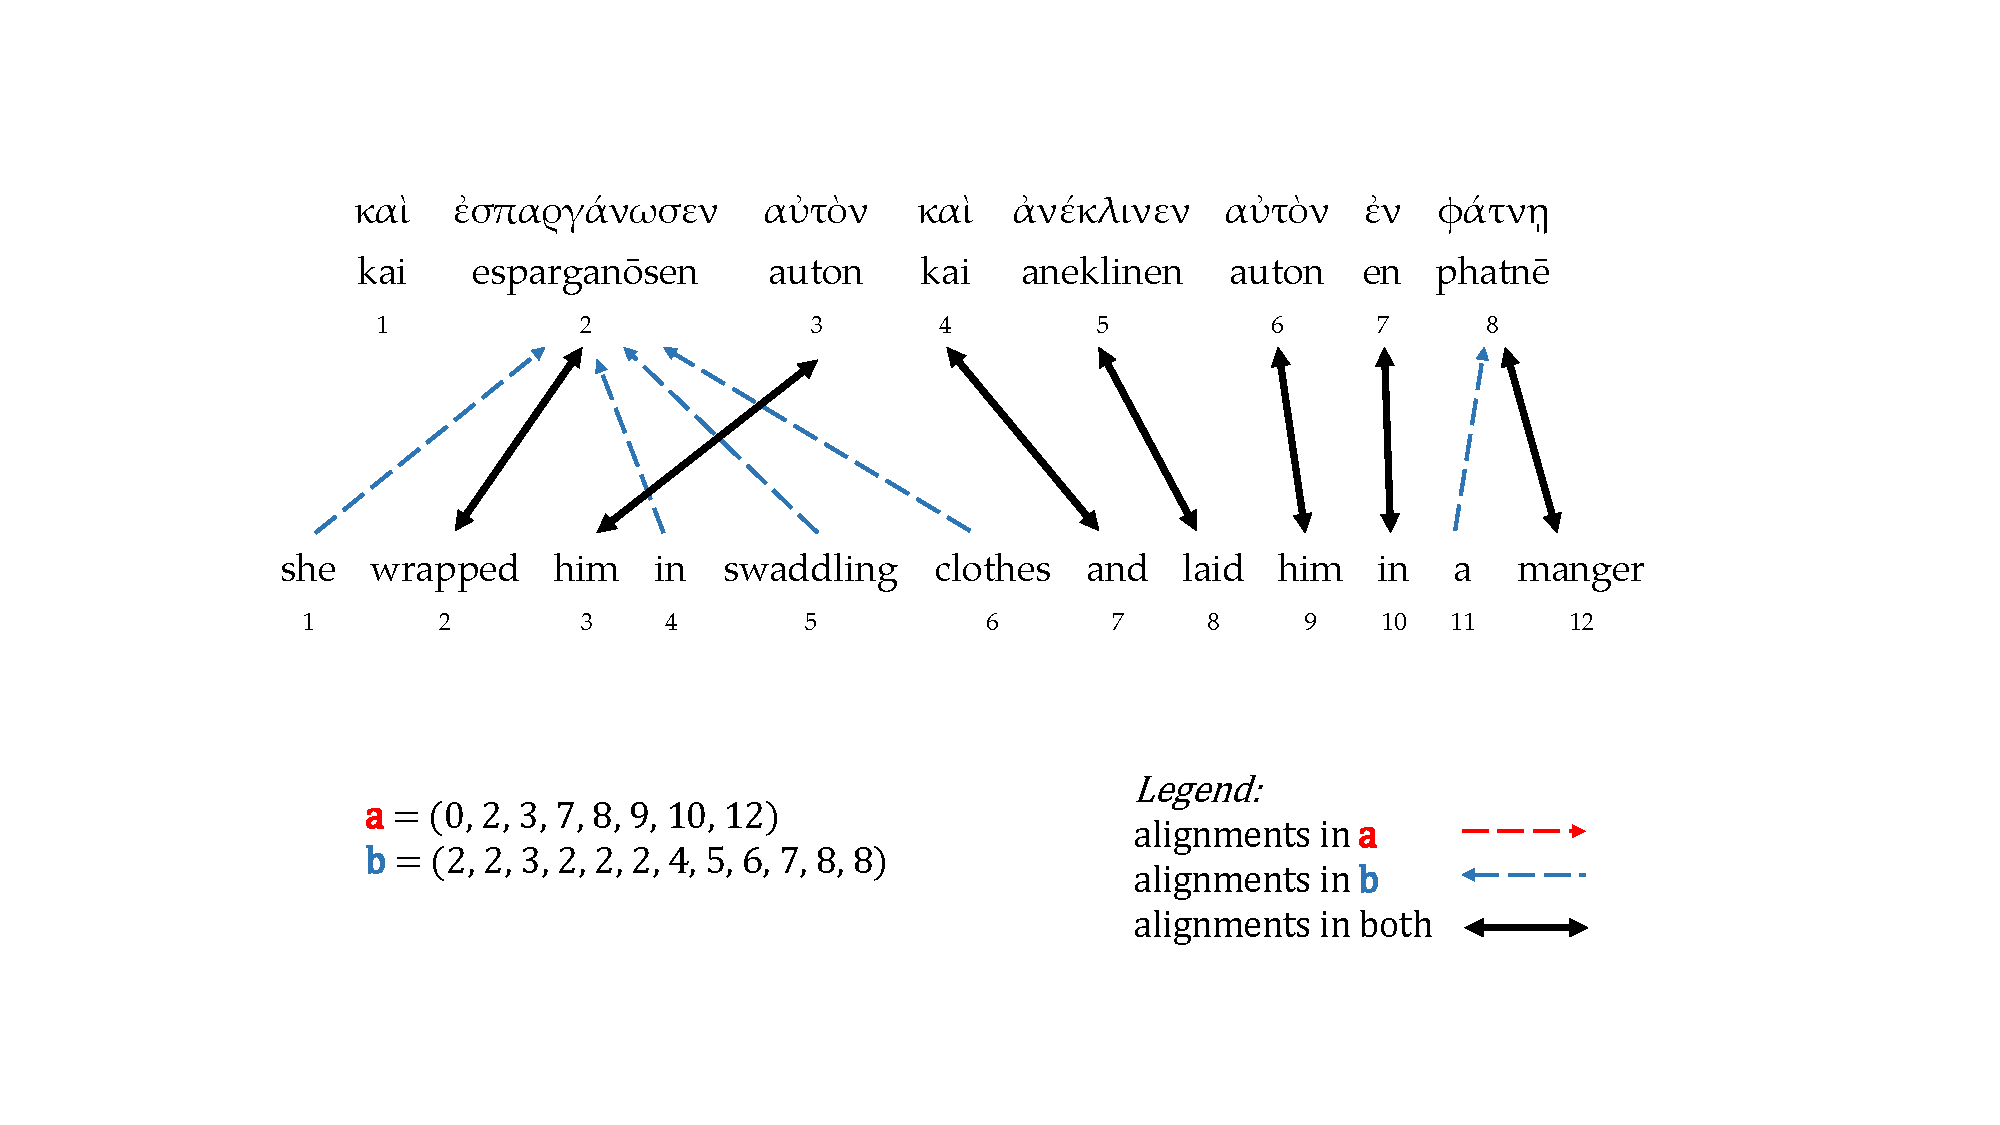
\includegraphics[scale=0.5]{phrase_align.pdf}
\caption{An example of a two-pass alignment between Greek and English.}
\label{phrase_align}
\end{figure}

There is a problem here: which values from $\aa$ and $\bb$ should determine $A$?
The matrix could be built such that $A(i,j) = 1$ whenever $a_j = i$, or perhaps also when $b_i = j$, (the union), which
would be sensible because one-to-many alignments can be found only from the reverse direction.
Or, by a stricter rule, both $a_j = i$ and $b_i = j$ could be required so that the alignments reinforce one another (the intersection).
If $A$ contains too many or too few word alignments it will not be informative.

The solution is to use heuristics \cite{och:99, koehn:03}.
Most of these begin by adding all of the word alignments from the intersection
and then iteratively adding some of the word alignments from the union according to some rule. 
Koehn \cite{koehn:03} finds experimentally that the best rule is generally to fill by adding an alignment
from the union only if:

\begin{enumerate}
\item both words are adjacent to a word already aligned or are already aligned themselves
\item at least one of the words has no previous alignments in the table.
\end{enumerate}

Och's original heuristic is similar but allows only one adjacent word \cite{och:99, och:00, och:04} (see Figure \ref{heuristic}). 

From Figure \ref{phrase_align} we also see that this method of generating many-to-many alignments by performing many-to-one alignments
in both translation directions cannot generate arbitrary many-to-many alignments.
For example, we might reasonably want to connect English \textit{she} to both Greek verbs, \textit{espargan\={o}sen} and \textit{aneklinen},
since the pronoun in English is construed by the conjugation of the verb in Greek.
To do this within our method, we would need to connect both Greek verbs to \textit{she} from the Greek-to-English direction.
But these verbs are already aligned to the corresponding English verbs.
So ours is a jealous alignment -- any source language words participating in a one-to-many alignment cannot be aligned to
anything else.

\begin{figure}
\centering
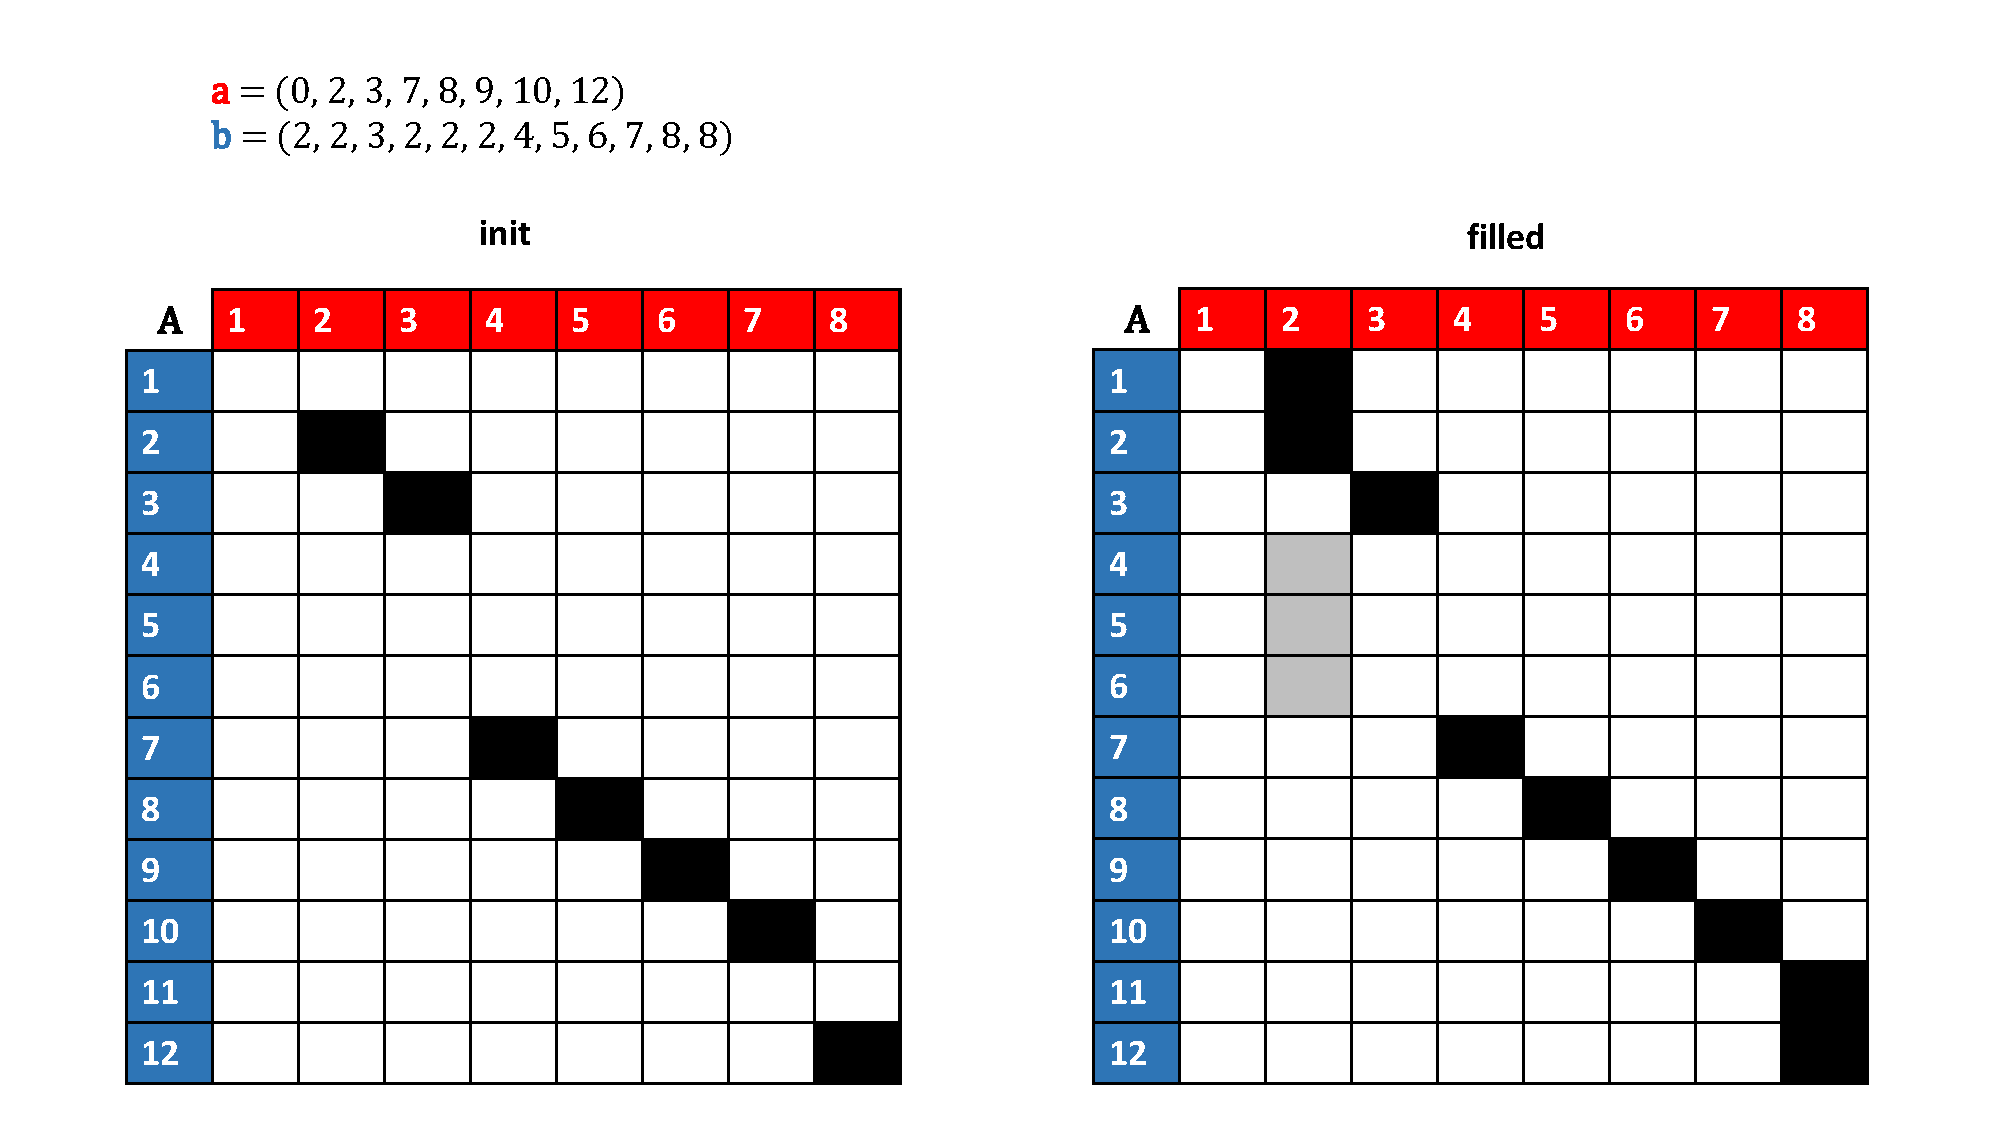
\includegraphics[scale=0.5]{heuristic.pdf}
\caption{Filling the alignment matrix $A$ by heuristic. The gray squares ($A(4:6,2)$) are filled by Koehn's heuristic but not by
Och's. Note that the matrix filled by Koehn's heuristic contains all of the word alignments.}
\label{heuristic}
\end{figure}

With this done, phrase-based alignment is a trivial step away: we say that two phrases are aligned
if and only if their constituent words align only to each other \cite{och:99}.
Note that ``phrase'' is not being used in any linguistic sense here; it is synonymous with ``$n$-gram.''
For example, \textit{house the} might be a phrase picked up by the model \cite{chiang:05}.
The model can again be trained with EM with the alignment table as a hidden variable \cite{och:99}.

% Koehn, Och, Marcu (2003)

% Recent research: neural nets

\subsection{Phrase-Based Systems}
Koehn et al.\ replicated Och's results and produced the freely available
``Pharaoh'' system for phrase-based SMT, released in 2004 \cite{koehn:03, pharaoh}.
Pharaoh was later made into an open-source project and was renamed ``Moses\footnote{The 
Egypt-related names harken back to the GIZA and Cairo SMT tools, which were free implementations
of the IBM Models \cite{giza, cairo}.},'' released in 2007 \cite{moses}.
These systems quickly supplanted IBM's word-based methods as
the state-of-the art and are frequently used as baselines for evaluating new models \cite{lopez, chiang:05}.

\section{Parse-Based Models}
\subsection{Phrases of Phrases}
% Hierarchical phrase-based, aka parse-based
As Chiang shows, phrase-based models like Pharaoh do a fine job of finding phrases
but often reorder them haphazardly in translation \cite{chiang:05}. This problem is called
``phrase salad'' \cite{lopez}. 
This is especially a problem between structurally dissimilar languages like 
English and Chinese or Japanese.

% Yamada and Knight (2001)
One solution to this is to parse the input language and build a parse tree \cite{yamada_knight}.
Then, instead of reordering individual words, whole nodes in the tree are reordered
with probabilities conditional on the nodes' parents and children (i.e.\ their syntactic context).
The leaf nodes (the actual words in the source language) are translated as usual.
Note that this method, while using phrasal information to perform long-distance reorderings more coherently,
still produces a word-based alignment.

While this is an intuitively appealing approach, it requires a reliable syntactic parser for 
the source language and such parsers are available only for a small number of well-studied languages \cite{lopez}.
Furthermore, parsers may bereave our models of much of the flexibility that makes a statistical
approach appealing in the first place \cite{koehn:03}.

% Chiang(2005, 2007)
There is a compromise: a model can infer rules for a context-free grammar
from the corpus just as it infers alignments \cite{chiang:05, chiang:07}.
This is called ``parsing'' according to the formalism but it is not done in a linguistically informed fashion. 
Rather, it is simply a way of rewriting an input string, replacing some substrings by nonterminals and 
recursively applying the same procedure to the rewritten string, learning a probability
for rewriting each pattern of terminals and nonterminals.
For this reason, the method is sometimes called ``hierarchical phrase-based'' instead of ``parse-based.''
As Chiang describes it, ``since phrases are good for learning reorderings of words, we can use
them to learn reorderings of phrases as well'' \cite{chiang:05}.


% Kumar, Lopez summary -- parse-based models are formally more powerful, as we might expect
% but at what cost?

\subsection{Parse-Based Systems}
% Hiero
The system described in \cite{chiang:05} was released as ``Hiero'' in 2005 \cite{hiero}.
% Joshua
Following in Moses' tradition, the open-source Joshua toolkit was released in 2009,
bundling Hiero's functionality with a number of other modules for training and decoding
and an architecture designed for extensibility \cite{joshua}.
% NiuTrans
More recently, the NiuTrans system can learn either phrase-based or hierarchical phrase-based
language models and offers a variety of options for decoding \cite{niutrans}.
Unlike Joshua, which is written in Java with extensibility in mind,
NiuTrans is written in C++ for speed in training and decoding.

\section{Black-Box Analysis}
% compare and contrast the systems according to black-box
% and glass-box criteria (Dorr)
Each of these systems has particular strengths and weaknesses. Dorr et al.\ classify the rubrics 
for SMT systems into two groups \cite{dorr_survey}. Black-box criteria are concerned with how well the output matches
the input. Of course, the goodness of the output is not well-defined even for human translators,
so there are number of dimensions along which we can evaluate the fidelity of the output to the original text.

\subsection{Lexical Invariance}

There is one point that all current SMT models have in common by nature: \textit{lexical invariance}.
A translation is lexically invariant of its source when each of its words can be mapped directly
to a word in the source sentence \cite{dorr_survey}. Clearly, this is necessarily true
for all our systems because it follows directly from alignments, the Fundamental Equation of Machine Translation,
and learning translation probabilities from surface forms in bilingual corpora.
This is neither good nor bad in itself, but it does restrict the possible applications of SMT.
For example, there is no way an SMT system as currently formulated could produce, say, John Dryden's translation of the 
\textit{Aeneid}, which translates Virgil's dactylic hexameter into English rhyme schemes with consequent liberality in word choice.

\subsection{Alignment Quality}
The most immediate result by which the models can be evaluated is on the quality of their alignments or
phrase segmentations. Och and Ney \cite{och:00} describe a metric 
called \textit{alignment error rate (AER)} which combines precision and recall for auto-generated alignments
compared to handmade alignments, but the correctness of an alignment still relies on human judgment.

In general, phrase-based models are found to produce better alignments than word-based models.
Och and Ney's alignment template model outscores the IBM Model 5 on the quality of word alignments,
as does Yamada and Knight's syntax-based model.
This is an interesting observation: the alignment template model runs a word-based alignment
in both directions on the corpus (Och and Ney use a word-aligning Hidden Markov Model
comparable to the IBM Model 2 in power \cite{och:99, hmm}) and the alignments that were found in both passes
were kept, along with a few others found by a heuristic. So it seems that word-by-word
alignments benefit from simply running a second alignment and finding where they support each other.
This suggests that word-based methods inevitably produce some high-quality alignments which are consistently
generated and some spurious alignments that are simply noisy.

Pharaoh/Moses is effective at forming frequently adjacent words into phrases \cite{chiang:05}.
However, the grammars extracted from bilingual corpora by Hiero tend to lack the elegance and 
brevity of grammars formulated with linguistic knowledge. For example, the grammar extracted
in one of Hiero's evaluations contains around 24 million rules \cite{chiang:05}. 
This is a hurdle for decoding, which is already an NP-Hard problem on the size of the search space \cite{knight:99}.

\subsection{BLEU} \label{food-chain}
The introduction of BLEU \cite{bleu} scores in 2002 proved to be epochal. BLEU focuses on $n$-gram precision:
it rewards an output sentence for the number of words it matches with some reference output
and gives bonuses for matching $n$-grams of increasing length. 
Small BLEU scores go a long way: an increase of even 0.01 can be statistically significant \cite{koehn:03, chiang:05}.
However, it does not take overall word ordering into account and is therefore somewhat flattering towards phrase-based models.
Nevertheless, it is used widely for evaluation in SMT and many other NLP domains and 
has stimulated fruitful competition among researchers by providing an automatic, numerical scoring system \cite{lopez}.
Even today, BLEU remains the standard for black-box evaluation \cite{neural-nets}.

Koehn et al.\ carry out a thorough examination of word-based, phrase-based, and parse-based models 
to which they compare their own results \cite{koehn:03}. Using BLEU, they compare the translations
produced by these models as well as the translations produced by Pharaoh when varying certain parameters.
In general, the BLEU score increases exponentially with respect to the total number of words in the corpus.
Interestingly, longer phrases and more sophisticated word alignments do not produce better translations:
the BLEU scores stop improving past 3-grams and the IBM Model 2.
Pharaoh consistently beats the IBM Model 4 by about 0.02 BLEU. Even though Yamada and Knight's
syntax-based model beat the IBM Model 5 on alignment quality as evaluated by humans,
it was soundly beaten by the IBM Model 4 by around 0.03 BLEU and Pharaoh by 0.05 BLEU.

It is surprising that including syntactic information should degrade performance by so much.
Koehn et al.\ suspect that the parser is too restrictive: in their implementation, the parser
is simply a filter on the phrases on which translation probabilities are learned, and there
are simply too many possible syntactic parses for them all to appear in the corpus.
These tests were done without smoothing \cite{koehn:03}, so any unseen phrases
are assumed to have translation probability of zero -- a severe penalty.
Furthermore, not all translations are \textit{syntactically invariant},
especially those involving idioms \cite{dorr_survey, koehn:03}. In these cases, syntactic information would actually be misleading.

Actually, the syntax-based model that is tested in \cite{koehn:03} is not really the same one
that appears in \cite{yamada_knight}. In \cite{koehn:03}, the parser simply filters out
non-grammatical phrases like \textit{house the} from the model's parameters.
However, the real model is much more than that: in addition to learning probabilities
for translating individual words, it also learns probabilities for reordering syntax tree nodes
(the tree nodes are discarded in \cite{koehn:03}) and for inserting words in the output.
Furthermore, it still learns a translation probability independent of syntactic context for every word in the corpus,
so it is really much more robust than a model that filters out every ungrammatical phrase.
It was this model that outperformed the IBM Model 5 on the alignment task.
Even so, the criticisms are not entirely off the mark: requiring the input to conform
to a grammar will in fact present problems for some of the glass-box criteria.

Hiero puts the hierarchical phrase-based model at the top of the food chain by surpassing both Pharaoh
and alignment template system. In \cite{chiang:05}, Hiero scores about 0.02 BLEU higher than Pharaoh on a Chinese-English
task. In \cite{chiang:07}, it outperforms the alignment template system by about 0.03 BLEU, also in Chinese-English. 
Chinese to English translation, of course, requires many more reorderings of phrases than, say, French to English.
BLEU considers only local word order, but Chiang suggests that even this presents a difficulty to simple 
phrase-based systems in radically different languages \cite{chiang:05}.
Both Pharaoh and Hiero start with the same GIZA-generated word alignments,
so it is probable that Hiero performs better not because it is translating particular words differently but because it is scoring
more of BLEU's bonuses for longer $n$-gram matches.
Hiero also beats its previous results by quite a large margin -- 0.3457 BLEU against 0.2881 -- but the model in the later
paper is trained on a much larger dataset (28 million words against 10 million) and is combined with a stronger language model $\Pr(\ee)$.

\subsection{Speed}
Hiero flounders on a different black-box criterion: speed. 
Because of its more complex model, Hiero has more parameters to train and a much larger search space
(which is penalized exponentially as an NP-Hard problem). 
It does, in fact, use heuristics to make search faster but more errorful.
In 2005, Hiero takes about 20 seconds per sentence in decoding \cite{chiang:05}.
In 2007, Hiero is redesigned with faster language tools, is more sophisticated in pruning its search,
and is running on a faster processor \cite{chiang:07}.
However, its number of rules increases on its larger dataset: up from 2.2 million in 2005 (after filtering) to as high
as 5.5 million in 2007. Experiments are run to compare the effects of different degrees of pruning
on the BLEU score. At the pruning level adopted for the rest of the evaluation, decoding takes 35 seconds and achieves
0.3677 BLEU on average, after which the marginal increase in BLEU asymptotes.
While the other authors do not cite speed measurements for their models, Chiang mentions qualitatively that flat phrase-based
models translate considerably faster than Hiero \cite{chiang:07}.

\subsection{Semantic Invariance}
The ultimate goal of machine translation is \textit{semantic invariance}.
A statistical translation system enforces this at a very local level by nature because 
the word substitutions made by the system are consistent with the substitions
made in the training data. Assuming that the domain is sufficiently restricted for minimal lexical ambiguity, the output sentence
should at least consist of a number of correct words, though possibly in the wrong order.
This is promising, however, because we can completely sidestep the need for 
real-world knowledge and deep semantic understanding if the model can just find a way to get the words in the right
order. Phrases can do this locally to about three words \cite{koehn:03}, and applying phrases recursively can
bootstrap this even higher \cite{chiang:05}. Unfortunately, getting real data for evaluating semantic invariance
requires the opinions of experts and is usually bypassed for numerical, automatic scoring by BLEU.
With more mature models and increasing expectations
from users, perhaps it is time for the state-of-the-art to be held to standards of semantic invariance.

\section{Glass-Box Criteria}
Glass-box criteria judge the system on how well it adheres to good software design principles,
how reproducible its results are when trained on other corpora or when its modules are reimplemented,
and on how useful it is to future research \cite{dorr_survey}.

\subsection{Generality}
A major strength of the statistical approach in general is that it requires no
explicit linguistic information \cite{brown:93}. Today, bilingual corpora can be
easily assembled through the Internet and used to train a translation model.
In theory, the same statistical model, if good enough, may one day be able to provide translation
between arbitrary language pairs,
while a linguistic approach must formulate rules for analyzing every existing language. Furthermore,
the statistical approach is fault-tolerant and will still produce a result if the input has 
spelling or grammatical errors. Furthermore, certain domains, such as those involving spoken language
(if we are combining translation with speech recognition, for example), resist rigid linguistic accounts \cite{och:99}.

Even though Yamada's and Chiang's parse-based models are similar in motivation, Chiang's Hiero system
succeeds because it does not compromise its statistical groundings. By learning grammar rules
directly from the corpus, Hiero is not confined to any set of predefined rules and can readily adapt
to difficult or unconventional grammar.


\subsection{Extensibility}
As section \ref{food-chain} on BLEU shows, researchers are constantly reworking and improving their designs
to surpass the current state of the art. Extensibility comes in two types: building new strengths
and strengthening old weaknesses.

The choice of programming language and a modular architecture can make it easy to revise code and add new features.
Hiero was originally written in Python, a language that emphasizes readability and flexibility at the
efficiency cost of being interpreted \cite{chiang:05}. Hiero was later partially refactored into
Pyrex, a compiled superset of Python with C-style type declarations \cite{chiang:07}. 
Meanwhile, Joshua is written in Java with extensibility as an expressed goal of its modular, object-oriented
design \cite{joshua}.

A strength cited by Yamada and Knight \cite{yamada_knight} of their parse-based method is that a few of their
test sentences accounted for a disproportionate amount of errors. This is desirable
because most of the sentences will contain only high-quality alignments and because it also gives a clear indication of 
what can be improved in future work.

Making translation software open source allows other researchers to improve on the design.
Lopez cites the availability of open source toolkits for statistical translation as a major catalyst
for research in the late 2000s \cite{lopez}.
The Pharaoh system was originally free but closed source and was later replaced by Moses,
an open source version of the same design \cite{pharaoh, moses}.
Also, having high-quality free software proves to be helpful because more
complex systems often rely on simpler ones to accelerate their training (see section \ref{future}).
Distributing a free implementation of your system keeps other researchers
from having to reimplement it themselves, which saves their time and also ensures that your model will be fairly
represented when it is compared against other models.

\subsection{Scalability}
More sophisticated models with more parameters and larger data sets can improve the results of a translation
but may have substantial time and memory costs for training and decoding \cite{chiang:07}.
Hiero suffers from a lack of scalability because of the large increase in grammar rules with the size of the
dataset. Since this exponentially increases the upper bound on the time needed for an optimal search,
it must prune the search space and return a sub-optimal result, nullifying the benefit of a more complex model.

Besides using more efficient algorithms and data structures and a compiled language instead of an interpreted one,
a scalable SMT system should have a parallelized architecture
so training and decoding can be done concurrently on multiple CPUs. 
All of these considerations are made in the design of Joshua \cite{joshua}, which mitigate the added complexity
of its hierarchical phrase-based model.

\subsection{Utility to Future Research} \label{future}
Perhaps all of the glass-box criteria can be summarized by the following question: \textit{How useful is this system to posterity?}
A remarkable feature of all of the translation models discussed is that they all build off one another.
This is not just matter of inspiration and propagating ideas -- each system relies on an actual implementation
of one of the previous models to bootstrap its parameters during training. 

First, the IBM Models 1 and 2, which
make liberal and unrealistic independence assumptions, are formulated to make EM fast so their parameters
can be used as the initial guesses of more sophisticated Models 3, 4, and 5 \cite{brown:93}. 
The GIZA++ implementation of the IBM models \cite{giza} is used extensively in the phrase-based models to find word-by-word alignments.
Pharaoh, Moses, Joshua, and Hiero all use GIZA++ in their two-way pass through the corpus to find phrase alignments \cite{koehn:03, pharaoh, moses, joshua, chiang:05}.
Och and Ney bootstrap their alignment template models with a word-by-word Hidden Markov Model comparable to the IBM Model 2 in performance \cite{och:99}.
GIZA++, released in 2000, is actually the work of Och and Ney themselves, but interestingly they continue to use the HMM \cite{och:00, giza, och:04}.
Perhaps this is because better word-based alignments do not necessarily translate to better phrase alignments,
so a cheaper model is favorable for bootstrapping \cite{koehn:03}. 

\section{Conclusion}
% summary

Beginning with Och et al.'s alignment template model \cite{och:99}, phrase-based models
are very natural extensions of the original IBM Models. The prospect of coupling
the promising results of statistical methods with the arsenal of linguistic techniques
that had been applied to translation in the past was enticing from the beginning \cite{brown:93},
but attempts at including explicit information failed because they reneged on
SMT's promises of flexibility and generality \cite{yamada_knight, koehn:03}.
Models that do use parsing do not use prewritten linguistic rules but
rather grammars of their own creation, and these approaches have been successful \cite{chiang:07, joshua}.
Meanwhile, a number of open-source implementations of the most popular phrase-based models
continue to stimulate research and advancement \cite{moses, joshua}.

% What can be done to address the weaknesses?
% How can we take advantages of the strengths?
End-to-end translation systems are complicated software and require
much more than statistical and algorithmic considerations to be effective.
Perhaps the most important design decision is to make the system parallelizable
to take advantage of larger datasets in training and return more optimal
search results in decoding for the time taken. Furthermore, models and systems
must be designed so that they can be easily used and improved by their own architects
and other researchers.

\subsection{Future Directions}
Following general trends in artificial intelligence, phrase-based translation is being adapted
to use discriminative models \cite{chiang:07} and deep learning \cite{neural-nets} with promising results.
At the same time, these begin to diverge from the approach originally taken by the IBM Models,
where translation was formulated as a generative model.
And as NLP becomes increasingly prevalent in smartphones and on the Internet, machine translation
systems will need integrate with other NLP technology like speech recognition and adapt
to the special domains of typed or spoken input.
Phrase-based models may be particularly adept at matching common search terms
and the creative figures of speech that spontaneously arise from everyday speech and on the Internet.

% Morphology
Brown et al.\ anticipate in 1993 that including linguistic information for morphology 
promises the greatest improvements and should be the primary direction of future research \cite{brown:93}. 
Koehn notes in 2005 that this interesting problem remains neglected because most translation research takes
English, a morphologically poor language, as its target \cite{europarl}.
However, even the parsing-based models seem unequipped to handle this.
Yamada and Knight's syntax-based model uses the linguistic context to reorder phrases,
but the actual translations of the leaf nodes depend only on their identities and are
independent of their grammatical context \cite{yamada_knight}.
None of the authors address the suitability of their models for morphologically variant
language pairs.

Even in English, whose nouns and verbs inflect very little, there is opportunity for using morphological information.
Morphological analysis can identify suffixes for nouns (\textit{-ness}, \textit{-tion}, \textit{-ty}, 
\textit{-ment}, \textit{-or}, \textit{-er}), adjectives (\textit{-ous}, \textit{-wise}, \textit{-ant}), adverbs (\textit{-ly}),
and verbs (\textit{-ize}, \textit{-ed}). This, in turn, can be used in part-of-speech tagging or to 
extract word stems to reduce the size of the vocabulary and more accurately predict unseen forms
without smoothing. On the other hand, as with syntactic parsers, relying on morphological
information imposes restrictions on the possible source languages for the system.
Even so, this remains a ripe direction for future research.

\subsection*{Acknowledgments}
Thanks to Tamara Berg for her helpful direction and feedback.

\printbibliography

\end{document}
